\documentclass[11pt]{article}

% parameters are fairly self-explanatory here, thankfully
\usepackage[width=7in,height=9.5in,top=0.75in,centering]{geometry}

% for math-ing
\usepackage{amsmath}
\usepackage{amssymb}
\usepackage{comment}

%%%%%% tables %%%%%%%%

\usepackage{array}
\renewcommand{\arraystretch}{1.5}
\setlength{\tabcolsep}{8pt}

%%%%%% plotting %%%%%%

\usepackage[dvipsnames]{xcolor}
\usepackage{tikz}
\usepackage{pgfplots}

\pgfplotsset{every axis/.append style={
                    axis x line=middle,    % put the x axis in the middle
                    axis y line=middle,    % put the y axis in the middle
                    axis line style={<->,color=black}, % arrows on the axis
                    xlabel={$x$},          % default put x on x-axis
                    ylabel={$y$},          % default put y on y-axis
            }}
            
 \pgfplotsset{compat=1.14} % sometimes, everything falls apart without this
 
 %\usepgfplotslibrary{fillbetween} %for shading between curves

%%%%%% commands %%%%%%

% exam heading; course name is first argument, exam information is second argument
\newcommand{\Heading}[2]{
    \fbox{
        {\Large\textbf{#1}}
        }
    \hfill
    \fbox{
        \begin{minipage}{0.2\textwidth}
            \begin{center}
            \textbf{#2}
            \end{center}
        \end{minipage}
    }
    \par\vspace{0.1in}}

% for being lazy while beautifying integrals
\newcommand{\dint}{\displaystyle\int}

% for being lazy while beautifying limits
\newcommand{\dlim}{\displaystyle\lim}

%%%%%% stuff %%%%%%

\usepackage{fancyhdr}

%\setcounter{page}{0} % first page is page 0

\parindent0pt % no indent

\fboxsep=0.25cm % little space in fbox border

%%%%%% BEGIN! %%%%%%%

\begin{document}

\pagestyle{fancy}

% record goals here to create sense of transparency

\fancyhead[c]{%
  \ifcase\value{page}
  % empty test for page = 0
  \or {}% 
  \or
  \or {\bf\color{ProcessBlue} F1: Lines \& Slope}% page=1
  \or {\bf\color{RoyalBlue} L1: Limits and Continuity}% page = 2
  \or {\bf\color{RoyalBlue} L2: Evaluating Limits Using Continuity and Forms}% page = 3
  \or {\bf\color{ForestGreen} D1: Meaning of a Derivative}% page = 4
  \or {\bf\color{ProcessBlue} F2: Exponential and Logarithmic Functions}% page = 5
  \or {\bf\color{ForestGreen} D3: Derivatives of Basic Functions}% page = 7
  \or {\bf\color{ForestGreen} D2: Compute Derivatives}% page = 6
  \or {\bf\color{RedOrange} A1: Derivatives and Graphing}% page = 8
  \or
  \else
  % Empty chead here!
  \fi
}

\thispagestyle{empty} % don't display that this is page 0

\Heading{MATH 1190/1210 Survey of Calculus I}{Knowledge Checkpoint 2A\\Spring 2026}

\vspace{0.1in}

\textbf{Name} \hrulefill \, \begin{minipage}{0.16\textwidth}\begin{center}\textbf{UVA ID\\ (e.g. hdj4nd)} \end{center}\end{minipage}\hrulefill\\

\begin{minipage}{0.2\textwidth}\begin{center}\textbf{Course \&\\ Section Number} \end{center}\end{minipage} \hrulefill\,\,\textbf{Date} \hrulefill  \\

\hrulefill
\paragraph*{Course \& Section Numbers:}

{\small
\begin{center}
\begin{tabular}{| c | c | c | c |}
\hline
\begin{minipage}{0.12\textwidth}\centering
1190-100\\
J. Rolf\\
(2:00 PM)
\end{minipage}
&
\begin{minipage}{0.12\textwidth}\centering
1190-200\\
J. Rolf\\
(3:30 PM)
\end{minipage}
&
\begin{minipage}{0.12\textwidth}\centering
1190-300\\
Michael\\
(11 AM)
\end{minipage}
&
\begin{minipage}{0.12\textwidth}\centering
1210-200\\
Susan\\
(9:30 AM)
\end{minipage}
\\ \hline
\begin{minipage}{0.12\textwidth}\centering
1210-300\\
Susan\\
(2 PM)
\end{minipage}
&
\begin{minipage}{0.12\textwidth}\centering
1210-400\\
Holden\\
(12:30 PM)
\end{minipage}
&
\begin{minipage}{0.12\textwidth}\centering
1210-500\\
Susan\\
(3:30 PM)
\end{minipage}
&
\begin{minipage}{0.12\textwidth}\centering
1210-700\\
Aaratrick\\
(2:00 PM)
\end{minipage}
\\ \hline
\begin{minipage}{0.12\textwidth}\centering
1210-800\\
J. Bowling\\
(3:30 PM)
\end{minipage}
&
\begin{minipage}{0.12\textwidth}\centering
1210-900\\
J. Bowling\\
(5 PM)
\end{minipage}
&
\begin{minipage}{0.12\textwidth}\centering
1210-930\\
Vadim\\
(11 AM)
\end{minipage}
\\
\cline{1-3}
\end{tabular}
\end{center}
}


{%\small

\paragraph*{Instructions:}

\begin{itemize}
    
    \item The regular time allowed for completing this assessment is \fbox{$80$} minutes.
    %\item This assessment is out of 50 points.\\
    \item This assessment contains one single-part or multi-part problem for each of the following targets: {\bf\color{ProcessBlue}F1}, {\bf\color{RoyalBlue}L1}, {\bf\color{RoyalBlue}L2}, {\bf\color{ForestGreen}D1}, {\bf\color{ProcessBlue}F2}, {\bf\color{ForestGreen}D3}, {\bf\color{ForestGreen}D2}, {\bf\color{RedOrange}A1}.
    \item On each problem, you will receive a score of Exceeds Expectations (5), Proficient (4), Almost (3), Developing (2), Emerging (1), or Not Yet (0). {\bf Please do not interpret your score as a percentage.}
    %\item You will have opportunities to reassess on the targets appearing on this assessment after the next {\bf 2} assessments.\\
    \item You may NOT use calculators, dictionaries, notes, phones, or any other kind of aid.
    \item Please write neatly. What cannot be read, cannot be graded.
    \item Carefully work out each problem and clearly indicate your final answer to every problem.
    \item Throughout, give the most descriptive answer possible. \textbf{For instance, ``DNE" will not be accepted when ``$=\infty$" is applicable.}
    %\item Please provide the most specific answer possible. For instance, if a limit does not exist because it goes to $\infty$ or $-\infty$, then specify this.
    \item Please use the methods discussed up to this point in the course. For example, any work based on l'H\^opital's Rule will not receive credit.
    \item \textbf{All work must be shown unless otherwise specified.} Partial credit will not be given if appropriate work is not shown.
    \item In particular, {\bf any answer appearing with no justification will receive no credit regardless of whether the answer was correct}, unless otherwise specified.
    \item Please first respond to the prompts on which you feel most proficient, then respond to others later.
    \item This booklet is printed double-sided. It contains 12 pages and 8 numbered problems.
    \end{itemize}
    
    }

\vfill


%%%%%%%%%
\newpage

This page is left blank intentionally.\\

Use this page if you need additional space to write your solutions to any problem. \\

If you wish this page graded, you must refer to this page on \textbf{the original page} of the problem. Otherwise, your grader will NOT consider your work on this page.

\newpage%
%%%%%%%%%


\begin{enumerate}

%%%%%%%%%%%%%%%%%%%%%%%%%%%%%%%%%%%%%%%%%%%%%%%%%%%%%
%%%%%%%%%%% BEGIN PROBLEM F1 %%%%%%%%%%%%%%%%%%%%%%%%
%%%%%%%%%%%%%%%%%%%%%%%%%%%%%%%%%%%%%%%%%%%%%%%%%%%%%

\item A team of biologists is doing a long-term study of the population of rabbits on a small island. They perform population estimates every five years, and have collected the data shown below:

\[
    \begin{array}{|c|ccccc|}
        \hline\text{Year} & 2005 & 2010 & 2015 & 2020 & 2025\\\hline
        \text{Rabbit Population (thousands)} & 2.0 & 3.0 & 8.0 & 15 & 12\\\hline
    \end{array}
\]

\bigskip

\begin{enumerate}
    \item What is the net change in the population of rabbits on this island over the course of the study? (Be sure to include units.)

    \vspace{3cm}

        \,\hfill units: \rule{1.75in}{0.4pt}\\

    \item What is the average rate of change (AROC) of the population of rabbits on this island over this time frame?

    \vspace{3cm}

        \,\hfill units: \rule{1.75in}{0.4pt}\\

    \item Using your answer from part (b), give an educated guess for the total population of rabbits on the island in 2027. Explain your reasoning.
    

\end{enumerate}

%%%%%%%%%%%%%%%%%%%%%%%%%%%%%%%%%%%%%%%%%%%%%%%%%%%%%
%%%%%%%%%%% END PROBLEM F1 %%%%%%%%%%%%%%%%%%%%%%%%%%
%%%%%%%%%%%%%%%%%%%%%%%%%%%%%%%%%%%%%%%%%%%%%%%%%%%%%

\newpage

%%%%%%%%%%%%%%%%%%%%%%%%%%%%%%%%%%%%%%%%%%%%%%%%%%%%%
%%%%%%%%%%% BEGIN PROBLEM L1 %%%%%%%%%%%%%%%%%%%%%%%%
%%%%%%%%%%%%%%%%%%%%%%%%%%%%%%%%%%%%%%%%%%%%%%%%%%%%%
\item Sketch the graph of a function $f(x)$ which satisfies all of the following:

\begin{enumerate}
    \item[(i)] $f(x)$ has a jump discontinuity at $x=-2$.
    \item[(ii)] $f(0)$ and $\displaystyle\lim_{x\to 0}f(x)$ both exist, but $f(x)$ is discontinuous at $x=0$.
    \item[(iii)] $\displaystyle\lim_{x\to 2^-}f(x) = -\infty$.
    \item[(iv)] $f(x)$ is defined on all of $[-3,3]$, and is discontinuous only at $x=-2$, $x=0$, and $x=2$.
\end{enumerate}

\vspace{2cm}

\begin{center}
    \begin{tikzpicture}[scale=1]
    \begin{axis}[
    xlabel={$x$},
    xtick = {-3,-2,-1,1,2,3},
    xticklabels = {$-3$, $-2$,$-1$,$1$, $2$, $3$},
    ylabel={$y$},
    ytick = {-3,-2,-1,1,2,3},
    yticklabels = {$-3$, $-2$,$-1$,$1$, $2$, $3$},
    samples=160,
    domain=-1:3,
    xmin=-3.5, xmax=3.5,
    ymin=-3.5, ymax=3.5,
    grid=both, grid style=dashed,
    width=5.4in, height=5.4in
    ]
    \end{axis}
    \end{tikzpicture}
\end{center}



\newpage

%%%%%%%%%%%%%%%%%%%%%%%%%%%%%%%%%%%%%%%%%%%%%%%%%%%%%
%%%%%%%%%%% END PROBLEM L1 %%%%%%%%%%%%%%%%%%%%%%%%%%
%%%%%%%%%%%%%%%%%%%%%%%%%%%%%%%%%%%%%%%%%%%%%%%%%%%%%

%%%%%%%%%%%%%%%%%%%%%%%%%%%%%%%%%%%%%%%%%%%%%%%%%%%%%
%%%%%%%%%%% BEGIN PROBLEM L2 %%%%%%%%%%%%%%%%%%%%%%%%
%%%%%%%%%%%%%%%%%%%%%%%%%%%%%%%%%%%%%%%%%%%%%%%%%%%%%
\item For each limit below, first determine the form of the limit, then find the value of the limit. 
If the given function is continuous at the target, you may simply write ``n/a'' for the form. 
Show complete work --- using mathematics and/or words --- to justify your answers. 
({\it Note:} $e \approx 2.718$.)


\begin{enumerate}
    \item[(a)] $\displaystyle\lim_{x\to\infty} \frac{e^{5x}+ \ln(x)}{x^{5} - 2}$
    \hspace{1cm}
    \textbf{form:} \rule[-6pt]{1.25in}{0.4pt} \quad
    \textbf{value:} \rule[-6pt]{1.25in}{0.4pt}
    \vspace{5cm}

    \item[(b)] 
        $\displaystyle\lim_{x\to0} \frac{\ln(1+x)-e^{2x}}{x-1}$
    \hspace{1cm}
    \textbf{form:} \rule[-6pt]{1.25in}{0.4pt} \quad
    \textbf{value:} \rule[-6pt]{1.25in}{0.4pt}
    \vspace{5cm}

    \item[(c)] 
    $\displaystyle\lim_{x\to 0^{+}} \frac{\sqrt{1+x}}{\ln(x)}$
    \hspace{1cm}
    \textbf{form:} \rule[-6pt]{1.25in}{0.4pt} \quad
    \textbf{value:} \rule[-6pt]{1.25in}{0.4pt}
    \vspace{0.3in}
\end{enumerate}

%%%%%%%%%%%%%%%%%%%%%%%%%%%%%%%%%%%%%%%%%%%%%%%%%%%%%
%%%%%%%%%%% END PROBLEM L2 %%%%%%%%%%%%%%%%%%%%%%%%%%
%%%%%%%%%%%%%%%%%%%%%%%%%%%%%%%%%%%%%%%%%%%%%%%%%%%%%

\newpage

%%%%%%%%%%%%%%%%%%%%%%%%%%%%%%%%%%%%%%%%%%%%%%%%%%%%%
%%%%%%%%%%% BEGIN PROBLEM D1 %%%%%%%%%%%%%%%%%%%%%%%%
%%%%%%%%%%%%%%%%%%%%%%%%%%%%%%%%%%%%%%%%%%%%%%%%%%%%%
\item A severe storm is passing over a city. The graph below shows total accumulated rainfall $R(t)$ (measured in inches), where $t$ is the number of hours since the storm started.

\begin{center}
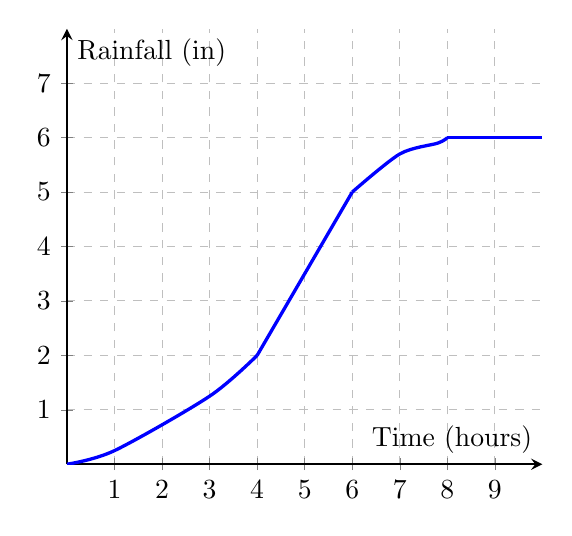
\begin{tikzpicture}
\begin{axis}[
    width=6cm,
    height=6cm,
    xmin=0, xmax=10,
    ymin=0, ymax=8,
    xtick={1,2,3,4,5,6,7,8,9},
    xticklabels={1,2,3,4,5,6,7,8,9},
    ytick={1,2,3,4,5,6,7},
    yticklabels = {1,2,3,4,5,6,7},
    xlabel={Time (hours)},
    ylabel={Rainfall (in)},
    axis lines=left,
    grid=both,grid style=dashed,
    width=3in, height=2.8in,
    thick
]

% First segment (varying speed)
\addplot[blue, very thick, smooth] 
coordinates {
(0,0)
(1,0.25)
(3,1.25)
(4,2)
};

% \addplot[domain=1:3, blue, very thick] {0.5*x-0.25};

% \addplot[blue, very thick, smooth] 
% coordinates {
% (3,1.25)
% (4,2)
% };

\addplot[domain=4:6, blue, very thick] {1.5*x-4};

\addplot[blue, very thick, smooth] 
coordinates {
(6,5)
(7,5.7)
(7.8,5.9)
(8,6)
};

\addplot[domain=8:10, blue, very thick] {6};

\end{axis}
\end{tikzpicture}
\end{center}

\begin{enumerate}
    \item Compute $R'(9)$. What does the value you get mean in this context?

    \vspace{3cm}

    \item Compute $R'(5)$. Be sure to include units.

    \vspace{2cm}
            \,\hfill units: \rule{1.75in}{0.4pt}\\
    
    \item The drainage infrastructure of the city is designed to handle rainfall rates up to $1$ inch per hour before starting to back up. At what time do you expect the highest risk of flooding? 
    
    \textbf{Justify your answer using the derivative.}

    (Note: there are multiple correct answers to this part; the important thing is that you demonstrate working knowledge of what the derivative means)
\end{enumerate}


%%%%%%%%%%%%%%%%%%%%%%%%%%%%%%%%%%%%%%%%%%%%%%%%%%%%%
%%%%%%%%%%% END PROBLEM D1 %%%%%%%%%%%%%%%%%%%%%%%%%%
%%%%%%%%%%%%%%%%%%%%%%%%%%%%%%%%%%%%%%%%%%%%%%%%%%%%%

\newpage

%%%%%%%%%%%%%%%%%%%%%%%%%%%%%%%%%%%%%%%%%%%%%%%%%%%%%
%%%%%%%%%%% BEGIN PROBLEM F2 %%%%%%%%%%%%%%%%%%%%%%%%
%%%%%%%%%%%%%%%%%%%%%%%%%%%%%%%%%%%%%%%%%%%%%%%%%%%%%

\item Respond to the following prompts. For this specific question, you are not required to compute any powers of constants or logarithms. For example, if your final answer includes $10^3$ or $\log_2(5)$, you can leave it as is.

\begin{enumerate}
    \item Simplify the expression below as much as possible so that the final result contains only positive exponents. You may expand exponential expressions and/or apply properties of exponents as needed. 

        \[
            \left(\frac{7x^{-1/3}}{2x^2}\right)^{-3}
        \]

    \vfill

    \item Solve the following equation for $x$. 

    \[\log_{5}(x) + \log_{5}(x - 4) = 1\]

    \vfill
     \item Solve the following equation for $x$. 

    \[7^{3x + 1} = 49^{5x}\]

    \vfill
\end{enumerate}


%%%%%%%%%%%%%%%%%%%%%%%%%%%%%%%%%%%%%%%%%%%%%%%%%%%%%
%%%%%%%%%%% END PROBLEM F2 %%%%%%%%%%%%%%%%%%%%%%%%%%
%%%%%%%%%%%%%%%%%%%%%%%%%%%%%%%%%%%%%%%%%%%%%%%%%%%%%

\newpage

%%%%%%%%%%%%%%%%%%%%%%%%%%%%%%%%%%%%%%%%%%%%%%%%%%%%%
%%%%%%%%%%% BEGIN PROBLEM D3 %%%%%%%%%%%%%%%%%%%%%%%%
%%%%%%%%%%%%%%%%%%%%%%%%%%%%%%%%%%%%%%%%%%%%%%%%%%%%%

\item Write down the derivatives of the following functions. No work required. No need to simplify.

If you need to write down your work, please do so at the bottom half of this page, not in the answer space.

\begin{center}
        \begin{tabular}{l c r l c r}
            %
            $\displaystyle\frac{d}{dx}\left[ -4x^{9} \right]$ & $=$ & \rule[-8pt]{1.5in}{0.4pt} &
            \vspace{4cm}
            %
            $\displaystyle\frac{d}{dx}\left[ \dfrac{2}{\sqrt{x^3}} \right]$ & $=$ & \rule[-8pt]{1.5in}{0.4pt}\\[0.3in]
            \vspace{4cm}
            %%%%%
            $\displaystyle\frac{d}{dx}\left[ 4^x \right]$ & $=$ & \rule[-8pt]{1.5in}{0.4pt} & 
            %%%%%
            $\displaystyle\frac{d}{dx}\left[ \frac{\pi^2}{6} \right]$ & $=$ & \rule[-8pt]{1.5in}{0.4pt}\\[0.3in]
            \vspace{4cm}
            %%%%%
            $\displaystyle\frac{d}{dx}\left[ x^2 + x+1 \right]$ & $=$ & \rule[-8pt]{1.5in}{0.4pt}&
            %
            $\displaystyle\frac{d}{dx}\left[ \ln(x) + x \right]$ & $=$ & \rule[-8pt]{1.5in}{0.4pt}\\[0.3in]
            \vspace{3cm}
            %%%%%
            $\displaystyle\frac{d}{dx}\left[ \log_2(x^5) \right]$ & $=$ & \rule[-8pt]{1.5in}{0.4pt} & 
            %
            $\displaystyle\frac{d}{dx}\left[ \frac{1}{x} + \frac{2}{x^2} \right]$ & $=$ & \rule[-8pt]{1.5in}{0.4pt}\\[0.3in]
            %%%%%
        \end{tabular}
        
\end{center}


%%%%%%%%%%%%%%%%%%%%%%%%%%%%%%%%%%%%%%%%%%%%%%%%%%%%%
%%%%%%%%%%% END PROBLEM D3 %%%%%%%%%%%%%%%%%%%%%%%%%%
%%%%%%%%%%%%%%%%%%%%%%%%%%%%%%%%%%%%%%%%%%%%%%%%%%%%%

\newpage

%%%%%%%%%%%%%%%%%%%%%%%%%%%%%%%%%%%%%%%%%%%%%%%%%%%%%
%%%%%%%%%%% BEGIN PROBLEM D2 %%%%%%%%%%%%%%%%%%%%%%%%
%%%%%%%%%%%%%%%%%%%%%%%%%%%%%%%%%%%%%%%%%%%%%%%%%%%%%

\item Find the derivative of the following expressions. 

A correct final answer receives full credit. Nevertheless, you are encouraged to write down the steps so that you will be able to receive partial credit if you final answer is not fully correct. There's no need to simplify your final answer.

\begin{enumerate}
\item $\dfrac{(x^3 - x^2 +1)\ln(x)}{x}$

\vfill

\item $e^{3x}\left(x^4+3x\right)^7$

\vfill 
\end{enumerate}

%split part (a) and part (b)

%%%%%%%%%%%%%%%%%%%%%%%%%%%%%%%%%%%%%%%%%%%%%%%%%%%%%
%%%%%%%%%%% END PROBLEM D2 %%%%%%%%%%%%%%%%%%%%%%%%%%
%%%%%%%%%%%%%%%%%%%%%%%%%%%%%%%%%%%%%%%%%%%%%%%%%%%%%

\newpage

%%%%%%%%%%%%%%%%%%%%%%%%%%%%%%%%%%%%%%%%%%%%%%%%%%%%%
%%%%%%%%%%% BEGIN PROBLEM A1 %%%%%%%%%%%%%%%%%%%%%%%%
%%%%%%%%%%%%%%%%%%%%%%%%%%%%%%%%%%%%%%%%%%%%%%%%%%%%%

\item Consider the following function $f(x)$.

\[f(x)=x + \frac{1}{x^3}\]

Respond to the following prompts. Make sure to show all work.

\begin{enumerate}
    \item Find all critical numbers of $f(x)$.

    \vspace{6cm}

    \item On what interval(s) is $f(x)$ concave up? On what intervals(s) is $f(x)$ concave down?

    \vspace{6cm}

\end{enumerate}


%%%%%%%%%%%%%%%%%%%%%%%%%%%%%%%%%%%%%%%%%%%%%%%%%%%%%
%%%%%%%%%%% END PROBLEM A1 %%%%%%%%%%%%%%%%%%%%%%%%%%
%%%%%%%%%%%%%%%%%%%%%%%%%%%%%%%%%%%%%%%%%%%%%%%%%%%%%

\newpage

This page is left blank intentionally.\\

Use this page if you need additional space to write your solutions to any problem. \\

If you wish this page graded, you must refer to this page on \textbf{the original page} of the problem. Otherwise, your grader will NOT consider your work on this page.

\newpage

This page is left blank intentionally.\\

Use this page if you need additional space to write your solutions to any problem. \\

If you wish this page graded, you must refer to this page on \textbf{the original page} of the problem. Otherwise, your grader will NOT consider your work on this page.

\end{enumerate}

\end{document}